\section{Algorithm to solve $ n $ linear equation using pipeling}
\begin{figure}[!htbp]
    \centering
    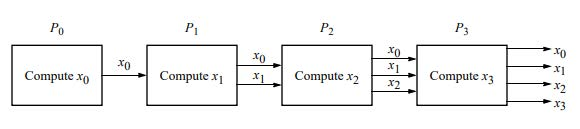
\includegraphics[width=\textwidth]{pipeline-linear-equation}
\end{figure}

\subsection{Sequential Implementation}
\begin{minted}{c}
// Seperate computation of X[0]
X[0] = B[0]/A[0][0]; 
for (int i = 1; i < n; i++) { // job for remaining ones
    int sum = 0;
    for (int j = 0; j < i; j++) {
        sum += A[i][j]*X[j];
    }
    X[i] = (B[i] - sum)/A[i][i];
}
\end{minted}

\subsection{Parallel Implementation}
\begin{minted}{c}
for (int i = 0; i < n -1; i++) {
    for (int j = 0; j < i; j++) { 
        recv(&X[j], P[i-1]);
        send(&X[j], P[i+1]);
    }
    int sum = 0;
    for (int j = 0; j < i; j++) {
        sum += A[i][j]*X[j];
    }
    X[i] = (B[i] - sum)/A[i][i];
    send(&X[i], Pi+1);
}
\end{minted}